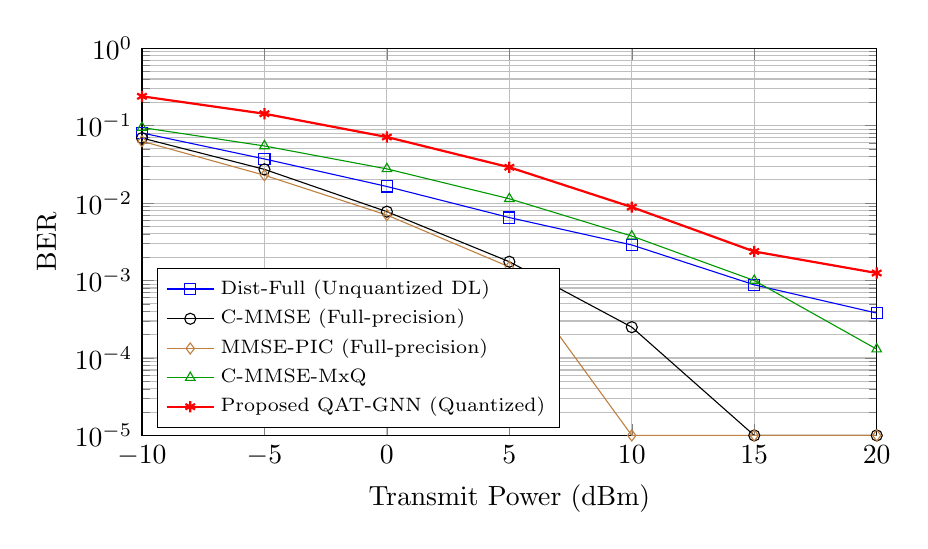
\begin{tikzpicture}
\begin{semilogyaxis}[
    width=0.9\linewidth,
    height=6.5cm,
    xlabel={Transmit Power (dBm)},
    ylabel={BER},
    xmin=-10, xmax=20,
    ymin=1e-5, ymax=1,
    grid=both,
    legend style={at={(0.02,0.02)},anchor=south west,font=\scriptsize},
    legend cell align={left}
]
\addplot[color=blue,mark=square] coordinates {
(-10, 0.08038) (-5, 0.03713) (0, 0.01638) (5, 0.00650) (10, 0.00288) (15, 0.00088) (20, 0.00038)
};
\addlegendentry{Dist-Full (Unquantized DL)}

\addplot[color=black,mark=o] coordinates {
(-10, 0.06913) (-5, 0.02725) (0, 0.00775) (5, 0.00175) (10, 0.00025) (15, 1e-5) (20, 1e-5)
};
\addlegendentry{C-MMSE (Full-precision)}

\addplot[color=brown,mark=diamond] coordinates {
(-10, 0.06288) (-5, 0.02287) (0, 0.00700) (5, 0.00150) (10, 1e-5) (15, 1e-5) (20, 1e-5)
};
\addlegendentry{MMSE-PIC (Full-precision)}

\addplot[color=green!60!black,mark=triangle] coordinates {
(-10, 0.09450) (-5, 0.05462) (0, 0.02763) (5, 0.01137) (10, 0.00375) (15, 0.00100) (20, 0.00013)
};
\addlegendentry{C-MMSE-MxQ}

\addplot[color=red,mark=asterisk,thick] coordinates {
(-10, 0.23900) (-5, 0.14238) (0, 0.07125) (5, 0.02900) (10, 0.00887) (15, 0.00237) (20, 0.00125)
};
\addlegendentry{Proposed QAT-GNN (Quantized)}
\end{semilogyaxis}
\end{tikzpicture}